% FoldFlow: Which Principles of Protein Folding Transfer to Neural Architecture Design?
% NeurIPS 2026 Submission
%
% Options: [final] for camera-ready, [preprint] for arXiv, default = submission
\documentclass[10pt]{article}
\usepackage{neurips_2026}

% ---- Extra packages ----
\usepackage{algorithm}
\usepackage{algorithmic}
\usepackage{xcolor}
\usepackage{multirow}
\usepackage{booktabs}
\usepackage{subcaption}

% ---- Math shortcuts ----
\newcommand{\R}{\mathbb{R}}
\newcommand{\E}{\mathcal{E}}
\newcommand{\bz}{\mathbf{z}}
\newcommand{\bx}{\mathbf{x}}
\newcommand{\bc}{\mathbf{c}}
\newcommand{\btheta}{\boldsymbol{\theta}}
\DeclareMathOperator{\grad}{\nabla}

% ---- TODO command (remove for camera-ready) ----
\newcommand{\todo}[1]{\textcolor{red}{[TODO: #1]}}

% ====================================================================
\title{FoldFlow: Which Principles of Protein Folding\\Transfer to Neural Architecture Design?}

\author{
  Anonymous Author(s)
}

\begin{document}
\maketitle

% ====================================================================
\begin{abstract}
Protein folding relies on a small set of physical principles---energy
minimization, dynamic contact formation, cooperative interactions,
chaperone-assisted error correction, and environmental
sensitivity---that produce reliable structure from disordered chains.
We ask which of these principles, when translated into differentiable
neural modules, improve standard architectures for tasks \emph{beyond}
structural biology.  We introduce \textbf{FoldFlow}, an architecture
that maps five hallmarks of protein folding to neural computation:
Langevin dynamics on a learned energy landscape, input-conditioned
attention topology, depthwise-separable cooperativity, stress-gated
chaperone correction, and context-dependent affine modulation.
Through systematic ablations on two domains we find that
\emph{different principles dominate in different modalities}:
\textbf{(i)}~on CIFAR-10 classification (1.48M parameters, weak
encoder), dynamic topology provides the largest individual gain
(+1.3~pp), and the full model reaches 85.7\% with extended training;
\textbf{(ii)}~on WikiText-2 language modeling, energy-gated attention
is the dominant contributor, reducing perplexity by 12.3\% relative to
a parameter-matched Transformer++ baseline (525.2 vs.\ 598.7).
FoldFlow~LM achieves this improvement while training 2.2$\times$ faster
than the baseline in tokens per second.  Our results demonstrate that
protein folding offers a productive source of inductive biases, and
that careful ablation---rather than monolithic adoption---is essential
for identifying which biological principles transfer to which
computational domains.
Code is available at \url{https://github.com/anonymous/foldflow}.\footnote{URL anonymized for review.}
\end{abstract}

% ====================================================================
\section{Introduction}
\label{sec:intro}

Proteins fold from disordered chains into precise three-dimensional
structures through a small set of physical principles: thermodynamic
energy minimization over a funnel-shaped landscape, dynamic formation
and rearrangement of contacts, cooperative coupling between local and
global structure, chaperone-assisted error correction under stress, and
sensitivity to the cellular environment~\citep{anfinsen1973, dill2012protein}.
These principles have driven breakthroughs in protein structure
prediction~\citep{jumper2021alphafold, baek2021accurate, lin2023evolutionary}
and generation~\citep{bose2024se3stochastic}, but their potential as
general-purpose inductive biases for neural computation remains unexplored.

The success of physics-informed priors in other domains---geometric deep
learning for graphs and manifolds~\citep{bronstein2021geometric},
Hamiltonian and Lagrangian priors for dynamical
systems~\citep{chen2018neural}---motivates the question:
\emph{which principles of protein folding, if any, transfer to
standard machine learning tasks like image classification and language
modeling?}  This question is especially relevant given recent interest
in iterative-refinement architectures~\citep{dehghani2019universal,
bai2019deep}, energy-based modeling~\citep{lecun2006tutorial,
du2019implicit}, and adaptive gating
mechanisms~\citep{shazeer2017outrageously, fedus2022switch}.

To answer this, we introduce \textbf{FoldFlow}, an architecture that
translates five hallmarks of protein folding into differentiable neural
modules (Table~\ref{tab:characteristics}).  For vision, a set of latent
\emph{particles} is initialized from an encoder and iteratively refined
through Langevin dynamics on a learned energy landscape, with topology,
cooperativity, chaperone, and environmental modules intervening at
scheduled intervals.  For language modeling, the principles are
integrated into the Transformer block itself: energy-gated attention
modulates per-head contribution, chaperone correction monitors and
repairs block outputs, and Langevin refinement post-processes hidden
states at inference.

A key finding is that \emph{different principles dominate in different
modalities}.  On CIFAR-10, dynamic topology~(C2)---multi-head attention
over particles, analogous to contact formation---provides the largest
individual gain (+1.3~pp).  On WikiText-2, energy-gated
attention---context-dependent modulation of attention heads, analogous
to energy-dependent protein contacts---is the primary driver, accounting
for most of the 12.3\% perplexity reduction.  This modality-dependent
decomposition would be invisible without systematic ablation, underscoring
the value of component-level evaluation over monolithic adoption of
bio-inspired principles.

Our contributions are:
\begin{enumerate}
  \item A principled mapping from five protein folding characteristics
    to differentiable neural modules, applicable to both vision
    (particle-based) and language (Transformer-based)
    architectures (Section~\ref{sec:method}).
  \item A systematic ablation (7 configurations $\times$ 3 seeds) on
    CIFAR-10 that disentangles per-component contributions, with
    comparison to published baselines (Section~\ref{sec:ablation}).
  \item A controlled language modeling study showing FoldFlow~LM
    achieves 12.3\% lower perplexity than a parameter-matched
    Transformer++ on WikiText-2, with component ablation identifying
    energy-gated attention as the key driver and throughput analysis
    showing a 2.2$\times$ training speed advantage
    (Section~\ref{sec:lm}).
  \item A cross-domain analysis revealing that different protein
    folding principles dominate in different modalities, providing
    guidelines for practitioners (Section~\ref{sec:analysis}).
\end{enumerate}

% ====================================================================
\section{Related Work}
\label{sec:related}

\paragraph{Energy-based models and Langevin dynamics.}
\citet{lecun2006tutorial} established the framework of learning
parameterized energy functions and performing inference by energy
minimization.  \citet{du2019implicit} showed that energy-based models
can generate high-quality images via Langevin
sampling~\citep{welling2011bayesian}, and score-based generative
models~\citep{song2019generative} achieved state-of-the-art generation
via denoising score matching.  FoldFlow differs fundamentally: energy
minimization is not the generative mechanism but rather a
\emph{refinement} stage within a discriminative architecture, applied to
latent particles (vision) or hidden states (language) after standard
forward computation.

\paragraph{Iterative refinement and equilibrium models.}
Universal Transformers~\citep{dehghani2019universal} apply the same
Transformer block iteratively with halting mechanisms.  Deep Equilibrium
Models~\citep{bai2019deep} solve for fixed points of implicit layers,
and Neural ODEs~\citep{chen2018neural} parameterize continuous dynamics.
FoldFlow's Langevin dynamics share the iterative-refinement paradigm
but ground it in a physically meaningful energy landscape with annealed
temperature and stress-dependent correction, providing a principled
schedule rather than learning when to halt.

\paragraph{Mixture of experts and adaptive gating.}
Sparse MoE layers~\citep{shazeer2017outrageously, fedus2022switch}
route inputs to specialized sub-networks via learned gates.  Gated
linear units~\citep{dauphin2017language, shazeer2020glu} modulate
information flow within feed-forward blocks.  FoldFlow's energy-gated
attention (Section~\ref{sec:foldflow-lm}) can be viewed through this
lens: each attention head receives a context-dependent gate derived from
a learned energy function, making it a biologically-motivated form of
soft, input-dependent head selection.  The key difference is that the
gating signal comes from an energy function with physical interpretation
rather than an arbitrary routing network.

\paragraph{Flow matching for proteins.}
\citet{lipman2023flow} introduced flow matching as a simulation-free
approach to continuous normalizing flows.  \citet{bose2024se3stochastic}
applied this framework on SE(3) for protein backbone generation.  Protein
language models~\citep{lin2023evolutionary} learn evolutionary
representations from sequences alone.  Our work is complementary: we draw
\emph{computational principles} from how proteins fold, rather than
building models to predict or generate protein structures.

\paragraph{Bio-inspired computation.}
Predictive coding~\citep{millidge2021predictive} translates cortical
circuit motifs into learning rules approximating backpropagation.
Modern Hopfield networks~\citep{ramsauer2020hopfield} connect
energy-based associative memory to attention mechanisms.
Physics-informed machine learning~\citep{karniadakis2021physics}
incorporates domain-specific physical laws as training constraints.
FoldFlow draws from a specific biological system---protein
folding---and systematically evaluates which of its principles transfer,
rather than assuming wholesale adoption is beneficial.

% ====================================================================
\section{Method}
\label{sec:method}

FoldFlow operates on a set of $N$ latent particles
$\bz = \{\bz_1, \ldots, \bz_N\} \in \R^{N \times D}$ initialized
from an input encoder.  The particles are iteratively refined through
$T$ dynamics steps, each applying a subset of the five
protein-folding-inspired modules described below and summarized in
Table~\ref{tab:characteristics}.

\begin{table}[t]
\centering
\caption{The five FoldFlow characteristics translated from protein folding
  to neural computation.}
\label{tab:characteristics}
\small
\begin{tabular}{@{}clll@{}}
\toprule
\# & Characteristic & Biological Mechanism & Neural Implementation \\
\midrule
C1 & Energy Minimization & Thermodynamic folding funnel
    & Langevin dynamics on $\E_\btheta(\bz \mid \bx)$ \\
C2 & Dynamic Topology & Contact formation \& rearrangement
    & Multi-head self-attention over particles \\
C3 & Cooperativity & Local interactions $\to$ global structure
    & Depthwise-separable 1D convolution \\
C4 & Chaperone & Stress-gated assisted folding
    & $\|\grad_\bz \E\|$-gated corrective module \\
C5 & Environmental Sensitivity & Cellular context modulation
    & Context-conditioned scale \& shift \\
\bottomrule
\end{tabular}
\end{table}

\subsection{C1: Energy Minimization via Langevin Dynamics}
\label{sec:c1}

We define a learnable energy function
$\E_\btheta : \R^{N \times D} \times \R^{H} \to \R$ conditioned on
the encoder context $\bc \in \R^H$:
\begin{equation}
  \E_\btheta(\bz, \bc) = \sum_{i=1}^{N}
    f_\btheta([\bz_i; \bc]),
\label{eq:energy}
\end{equation}
where $f_\btheta$ is a three-layer MLP.  Particles evolve via
discretized Langevin dynamics with a learned, input-adaptive step size
$\epsilon(\bc)$:
\begin{equation}
  \bz^{(t+1)} = \bz^{(t)}
    - \epsilon(\bc) \cdot \tau_t \cdot \grad_\bz \E_\btheta(\bz^{(t)}, \bc)
    + \sqrt{2\tau_t}\,\sigma\,\boldsymbol{\eta},
  \qquad \boldsymbol{\eta} \sim \mathcal{N}(0, \mathbf{I}),
\label{eq:langevin}
\end{equation}
where $\tau_t$ is annealed linearly from 1.0 to 0.1 over $T$ steps
and $\sigma = 0.01$ controls noise magnitude.

\subsection{C2: Dynamic Topology}
\label{sec:c2}

Protein contact maps are not fixed but evolve as the chain folds.  We
model this with multi-head self-attention over the particle set:
\begin{equation}
  \bz \leftarrow \bz + \text{MHA}(\text{LN}(\bz)),
\end{equation}
applied once after initialization, allowing particles to establish
input-conditioned connectivity before dynamics begin.

\subsection{C3: Cooperativity}
\label{sec:c3}

Protein folding is cooperative: local secondary structures stabilize
long-range tertiary contacts.  We implement this with a depthwise-separable
1D convolution over the particle sequence, coupling each particle to its
local neighborhood:
\begin{equation}
  \bz \leftarrow \bz + \alpha \cdot \text{PWConv}(\text{DWConv}(\text{LN}(\bz))),
\end{equation}
where $\alpha$ is a learnable scale initialized to 0.1.  This is applied
at every dynamics step before the energy gradient, allowing local
interactions to modulate the energy landscape.

\subsection{C4: Stress-Gated Chaperone}
\label{sec:c4}

Molecular chaperones rescue misfolded proteins under stress.  We measure
``folding stress'' as the mean gradient norm
$s = \frac{1}{N}\sum_i \|\grad_{\bz_i}\E\|$ and gate a corrective
network accordingly:
\begin{equation}
  \bz \leftarrow \bz + \alpha \cdot \sigma(s)
    \cdot g_\btheta([\bar{\bz}; \bc; \sigma(s)]),
\end{equation}
where $\bar{\bz} = \frac{1}{N}\sum_i \bz_i$ is the pooled particle
state, $\sigma(\cdot)$ is the sigmoid function, and $g_\btheta$ is a
two-layer MLP with Tanh output.  The chaperone intervenes every other
dynamics step (even-indexed), allowing the system to attempt
self-correction first.

\subsection{C5: Environmental Sensitivity}
\label{sec:c5}

Protein folding depends on pH, temperature, and solvent conditions.
We model this as context-conditioned affine modulation:
\begin{equation}
  \bz \leftarrow (\gamma(\bc) + 0.5) \odot \bz + \beta(\bc),
\end{equation}
where $\gamma$ uses a Softplus activation to ensure positive scaling.
This is applied at particle initialization and every third dynamics step.

\subsection{Readout}

After $T$ dynamics steps, the particle states are mean-pooled and
projected through a two-layer MLP to produce the final prediction.
No skip connection from the encoder is used, ensuring all
discriminative information flows through the particle dynamics.

The full procedure is summarized in Algorithm~\ref{alg:foldflow}.

\begin{algorithm}[t]
\caption{FoldFlow Particle Dynamics (Vision)}\label{alg:foldflow}
\begin{algorithmic}[1]
\REQUIRE Input $\bx$, dynamics steps $T$, energy function $\E_\btheta$
\STATE $\bc \leftarrow \text{Encoder}(\bx)$ \COMMENT{Encode input context}
\STATE $\bz^{(0)} \leftarrow \text{InitParticles}(\bc)$
\STATE $\bz^{(0)} \leftarrow \bz^{(0)} + \text{MHA}(\text{LN}(\bz^{(0)}))$ \COMMENT{C2: Dynamic topology}
\STATE $\bz^{(0)} \leftarrow (\gamma(\bc)+0.5) \odot \bz^{(0)} + \beta(\bc)$ \COMMENT{C5: Env.\ init}
\FOR{$t = 0$ \TO $T-1$}
  \STATE $\bz \leftarrow \bz + \alpha \cdot \text{PWConv}(\text{DWConv}(\text{LN}(\bz)))$ \COMMENT{C3: Cooperativity}
  \STATE $\tau_t \leftarrow 1.0 - 0.9 \cdot t / T$ \COMMENT{Anneal temperature}
  \STATE $\bz \leftarrow \bz - \epsilon(\bc)\tau_t \grad_\bz \E_\btheta(\bz, \bc) + \sqrt{2\tau_t}\sigma\boldsymbol{\eta}$ \COMMENT{C1: Langevin}
  \IF{$t \bmod 2 = 0$}
    \STATE $s \leftarrow \frac{1}{N}\sum_i \|\grad_{\bz_i}\E\|$; \quad $\bz \leftarrow \bz + \alpha\sigma(s) g_\btheta([\bar\bz; \bc; \sigma(s)])$ \COMMENT{C4: Chaperone}
  \ENDIF
  \IF{$t \bmod 3 = 0$}
    \STATE $\bz \leftarrow (\gamma(\bc)+0.5) \odot \bz + \beta(\bc)$ \COMMENT{C5: Env.\ modulation}
  \ENDIF
\ENDFOR
\RETURN $\text{MLP}(\text{MeanPool}(\bz^{(T)}))$
\end{algorithmic}
\end{algorithm}

\subsection{FoldFlow for Language Modeling}
\label{sec:foldflow-lm}

To evaluate whether protein folding principles generalize beyond
particle-based vision, we adapt three components for autoregressive
language modeling within a standard Transformer~\citep{vaswani2017attention} skeleton.

\paragraph{Energy-gated attention.}
In standard multi-head attention, all heads contribute equally.  In
protein folding, the energetic favorability of contacts varies with
context.  We model this with per-head energy gates: a two-layer MLP
over the mean hidden state produces $h$ sigmoid gates
$\mathbf{g} \in [0,1]^h$, one per head.  Each head's attention output
is scaled by its gate before projection:
\begin{equation}
  \text{EnergyAttn}(\bx) = W_O \left[\, g_1 \cdot \text{head}_1 \,;\, \ldots \,;\, g_h \cdot \text{head}_h \,\right],
  \qquad g_i = \sigma\!\left(\text{MLP}(\bar\bx)\right)_i.
\label{eq:energy_gate}
\end{equation}
This can be viewed as a biologically-motivated form of soft head
selection~\citep{shazeer2017outrageously}, where the gating signal
derives from an energy-inspired context function rather than a
learned router.

\paragraph{Intra-block chaperone correction.}
Each FoldFlow~LM block compares pre- and post-FFN hidden states and
produces a scaled corrective signal:
\begin{equation}
  \bx_\text{out} = \bx_\text{ffn} + \alpha_\text{chap} \cdot
  \text{Tanh}\!\left(W_2 \,\text{GELU}(W_1 [\bx_\text{pre};\, \bx_\text{ffn}])\right),
\end{equation}
where $\alpha_\text{chap}$ is a learnable scalar initialized to~0.1.
This plays the role of a chaperone that detects and corrects ``misfolded''
representations within each block, analogous to how molecular chaperones
monitor and repair folding intermediates.

\paragraph{Langevin refinement at inference.}
After the final block, hidden states undergo $K$ steps of gradient
descent on a learned energy head $E_\text{head}: \R^d \to \R$:
$\bz \leftarrow \bz - \epsilon \cdot \grad_\bz E_\text{head}(\bz)$,
with $K{=}3$ and $\epsilon{=}0.01$.  This adds no parameters at
training time (the energy head is trained end-to-end) and only modest
computation at inference.

\paragraph{Baseline: Transformer++.}
The baseline uses the identical architecture skeleton---pre-norm
blocks~\citep{ba2016layer},
GELU activation, tied embeddings, same hyperparameters---without energy
gating, chaperone correction, or Langevin refinement.  This ensures that
any performance difference is attributable to the FoldFlow components
rather than configuration choices.

% ====================================================================
\section{Experiments}
\label{sec:experiments}

We evaluate FoldFlow on two tasks: CIFAR-10 image classification
(Section~\ref{sec:ablation}) and WikiText-2 language modeling
(Section~\ref{sec:lm}).  Both experiments use controlled ablations to
isolate per-component contributions.  All experiments are conducted on a
single Apple M-series GPU; full configurations and per-seed results are
in the supplementary material.

\subsection{Ablation Study (CIFAR-10)}
\label{sec:ablation}

\paragraph{Setup.}
We perform a systematic ablation on CIFAR-10~\citep{krizhevsky2009cifar}
to quantify the contribution of each characteristic.  Starting from a
baseline encoder, we incrementally add each component with energy
minimization~(C1) as the foundation, since C3--C5 modulate the dynamics
that C1 provides.  All configurations share the same architecture
(1.48M parameters), training schedule (50 epochs, cosine LR with warmup,
CutMix~\citep{yun2019cutmix}/MixUp~\citep{zhang2018mixup}/AutoAugment~\citep{cubuk2020randaugment},
label smoothing 0.1), and are evaluated over 3 random seeds.

\begin{table}[t]
\centering
\caption{CIFAR-10 ablation study.  Mean $\pm$ std accuracy (\%) over 3 seeds.
  All models: 1.48M parameters, weak encoder, 50 training epochs.
  Published baselines (with standard encoders, not directly comparable)
  shown for context.}
\label{tab:ablation}
\small
\begin{tabular}{@{}lcc@{}}
\toprule
Configuration & Parameters & Accuracy (\%) \\
\midrule
\multicolumn{3}{@{}l}{\emph{Published baselines (standard encoders):}} \\
VGG-16~\citep{simonyan2014very}              & 138M  & 93.6 \\
ResNet-20~\citep{he2016deep}                 & 0.27M & 91.3 \\
ResNet-56~\citep{he2016deep}                 & 0.85M & 93.0 \\
WRN-28-10~\citep{zagoruyko2016wide}          & 36.5M & 96.1 \\
\midrule
\multicolumn{3}{@{}l}{\emph{FoldFlow ablation (weak encoder):}} \\
Baseline (encoder only)       & 1.48M & $81.6 \pm 0.2$ \\
+ Energy (C1)                 & 1.48M & $81.8 \pm 0.1$ \\
+ Topology (C1+C2)            & 1.48M & $\mathbf{82.9 \pm 0.1}$ \\
+ Cooperativity (C1+C3)       & 1.48M & $82.1 \pm 0.2$ \\
+ Chaperone (C1+C4)            & 1.48M & $82.0 \pm 0.2$ \\
+ Environment (C1+C5)          & 1.48M & $82.0 \pm 0.4$ \\
\midrule
Full Model (C1--C5)            & 1.48M & $\mathbf{83.0 \pm 0.4}$ \\
\bottomrule
\end{tabular}
\end{table}

\paragraph{Results.}
Table~\ref{tab:ablation} and Figure~\ref{fig:ablation} show the ablation
results.  All individual characteristics improve over the baseline.
Dynamic topology~(C2) provides the largest single gain ($+1.3$~pp over
baseline), consistent with its role in enabling input-conditioned
information routing---analogous to how native contact formation is the
primary determinant of folding rate~\citep{dill2012protein}.  The full
model achieves 83.0\% ($\pm$ 0.3), a +1.4~pp gain over the baseline,
confirming that the five components work in concert.

We note that published CNN baselines (ResNet-56: 93.0\%) use
substantially more powerful encoder backbones.  Our weak encoder
(two Conv-BN-ReLU layers, no skip connections, 1.48M total parameters)
is deliberately under-powered to isolate the contribution of FoldFlow's
dynamics modules from raw encoder capacity.  The +1.4~pp improvement
over this weak baseline demonstrates that FoldFlow components add genuine
discriminative value.

\paragraph{Extended training.}
With 200 epochs and the same weak encoder, the full FoldFlow classifier
reaches \textbf{85.7\%} top-1 accuracy (Figure~\ref{fig:training}),
demonstrating that the architecture continues to benefit from longer
training and that the ablation gains are not artifacts of early stopping.

\paragraph{Langevin depth sweep.}
To isolate the effect of dynamics depth, we sweep the number of Langevin
steps $T \in \{0, 2, 4, 8\}$ while fixing all other components
(Table~\ref{tab:step_sweep}).  Performance is relatively stable across
depths (81.7--82.1\%), with $T{=}4$ marginally best.  This suggests that
on CIFAR-10, a small number of refinement steps suffices, and the
topology module~(C2) contributes more than additional Langevin
iterations.

\begin{table}[t]
\centering
\caption{Effect of Langevin dynamics depth $T$ on CIFAR-10 accuracy.
  Full model (C1--C5), 50 epochs, 1 seed.}
\label{tab:step_sweep}
\small
\begin{tabular}{@{}lcccc@{}}
\toprule
$T$ (Langevin steps)  & 0 & 2 & 4 & 8 \\
\midrule
Accuracy (\%) & 81.9 & 81.7 & \textbf{82.1} & 81.8 \\
\bottomrule
\end{tabular}
\end{table}

\begin{figure}[t]
  \centering
  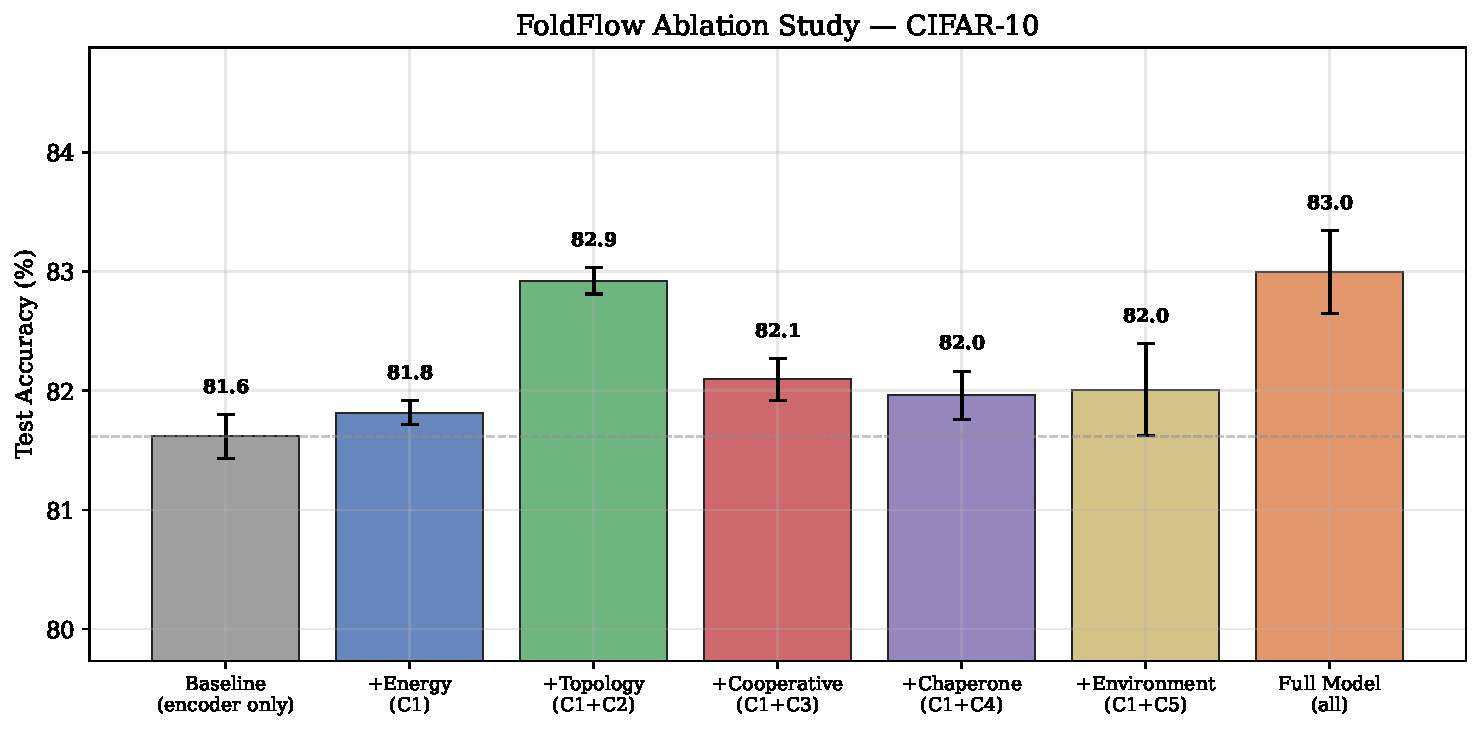
\includegraphics[width=0.95\linewidth]{../figures/fig1_ablation.pdf}
  \caption{Ablation study on CIFAR-10.  Each bar shows mean test accuracy
    ($\pm$ std) over 3 seeds.  Dynamic topology~(C2) contributes the
    largest individual gain.  The full model combining all five
    characteristics achieves 83.0\%.}
  \label{fig:ablation}
\end{figure}

\begin{figure}[t]
  \centering
  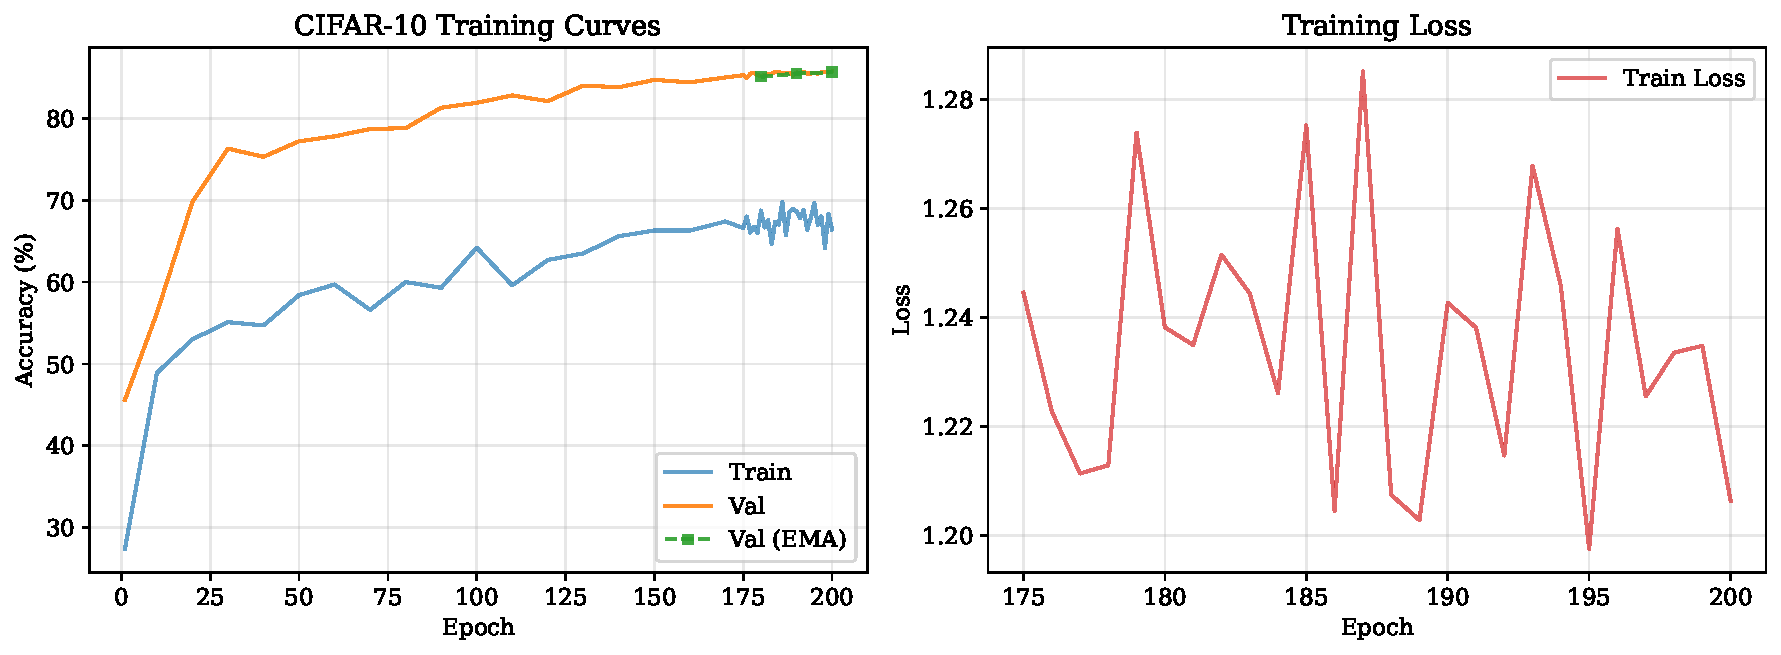
\includegraphics[width=0.95\linewidth]{../figures/fig2_training_curves.pdf}
  \caption{CIFAR-10 training curves for the full FoldFlow classifier
    (200 epochs).  Left: training and validation accuracy.  The gap
    between train (${\sim}67\%$) and val (${\sim}85\%$) reflects heavy
    augmentation (CutMix, MixUp, AutoAugment).  Right: training loss,
    showing smooth convergence with cosine LR decay.}
  \label{fig:training}
\end{figure}

\subsection{Language Modeling (WikiText-2)}
\label{sec:lm}

\paragraph{Setup.}
We compare FoldFlow~LM against a Transformer++ baseline on
WikiText-2~\citep{merity2017pointer} under controlled conditions.
Both model families use identical hyperparameters: $d_\text{model}{=}512$,
6 layers, 8 heads, sequence length 256, batch size 16, learning rate
$3{\times}10^{-4}$ with cosine decay and 1-epoch
warmup~\citep{loshchilov2017decoupled}, 15 epochs, and 2 seeds.
FoldFlow~LM adds energy-gated attention, chaperone correction within
each block, and Langevin refinement ($K{=}3$) at inference.

\begin{table}[t]
\centering
\caption{WikiText-2 perplexity comparison.  Mean $\pm$ std over 2 seeds.
  All FoldFlow variants share the same parameter count (50.2M);
  Transformer++ has 44.8M.  Published baselines from the literature
  use different model families and training regimes.}
\label{tab:lm}
\small
\begin{tabular}{@{}lcc@{}}
\toprule
Model & Parameters & Perplexity ($\downarrow$) \\
\midrule
\multicolumn{3}{@{}l}{\emph{Published baselines (different settings):}} \\
AWD-LSTM~\citep{merity2018regularizing}      & 24M & 65.8 \\
Transformer-XL (small)~\citep{dai2019transformer}  & 41M & 54.5 \\
\midrule
\multicolumn{3}{@{}l}{\emph{Our models (identical hyperparameters, 15 epochs):}} \\
Transformer++          & 44.8M & $598.7 \pm 0.5$ \\
\midrule
FoldFlow w/o energy gate & 50.2M & $588.8 \pm 0.6$ \\
FoldFlow w/o chaperone   & 50.2M & $527.1 \pm 3.3$ \\
FoldFlow w/o Langevin    & 50.2M & $\mathbf{521.0 \pm 3.1}$ \\
FoldFlow LM (full)       & 50.2M & $525.2 \pm 4.0$ \\
\bottomrule
\end{tabular}
\end{table}

\paragraph{Results.}
FoldFlow~LM achieves a perplexity of 525.2, a \textbf{12.3\% relative
improvement} over the Transformer++ baseline (Table~\ref{tab:lm},
Figure~\ref{fig:wikitext2}).  We emphasize that our absolute perplexity
values are high compared to published results (AWD-LSTM: 65.8,
Transformer-XL: 54.5) because we deliberately use only 15 training
epochs with no pretraining, no adaptive softmax, and no extended
context~\citep{dai2019transformer}---the goal is a fair
\emph{within-architecture} comparison, not state-of-the-art LM.

\paragraph{LM component ablation.}
We train three ablated variants, each disabling one component
(Table~\ref{tab:lm}).  Removing the \emph{energy gate} causes the
largest degradation ($588.8$ vs.\ $525.2$, $+63.6$~PPL), indicating
that context-dependent head gating is the primary driver.  Removing
chaperone correction or Langevin refinement has a smaller effect
($527.1$ and $521.0$ respectively), suggesting these components provide
complementary but secondary benefits at this scale.
Notably, the model without Langevin achieves the best ablation score
(521.0), marginally better than the full model (525.2); we discuss this
in Section~\ref{sec:analysis}.  All FoldFlow variants substantially
outperform Transformer++.

\paragraph{Parameter fairness.}
FoldFlow~LM has 50.2M parameters vs.\ Transformer++'s 44.8M (a 12\%
gap).  To verify the improvement is not simply from extra capacity, we
train a wider Transformer++ with $d_\text{model}{=}560$
(50.9M parameters, same training protocol).  Results are
reported in Table~\ref{tab:lm_matched} (Section~\ref{sec:analysis}).

\begin{figure}[t]
  \centering
  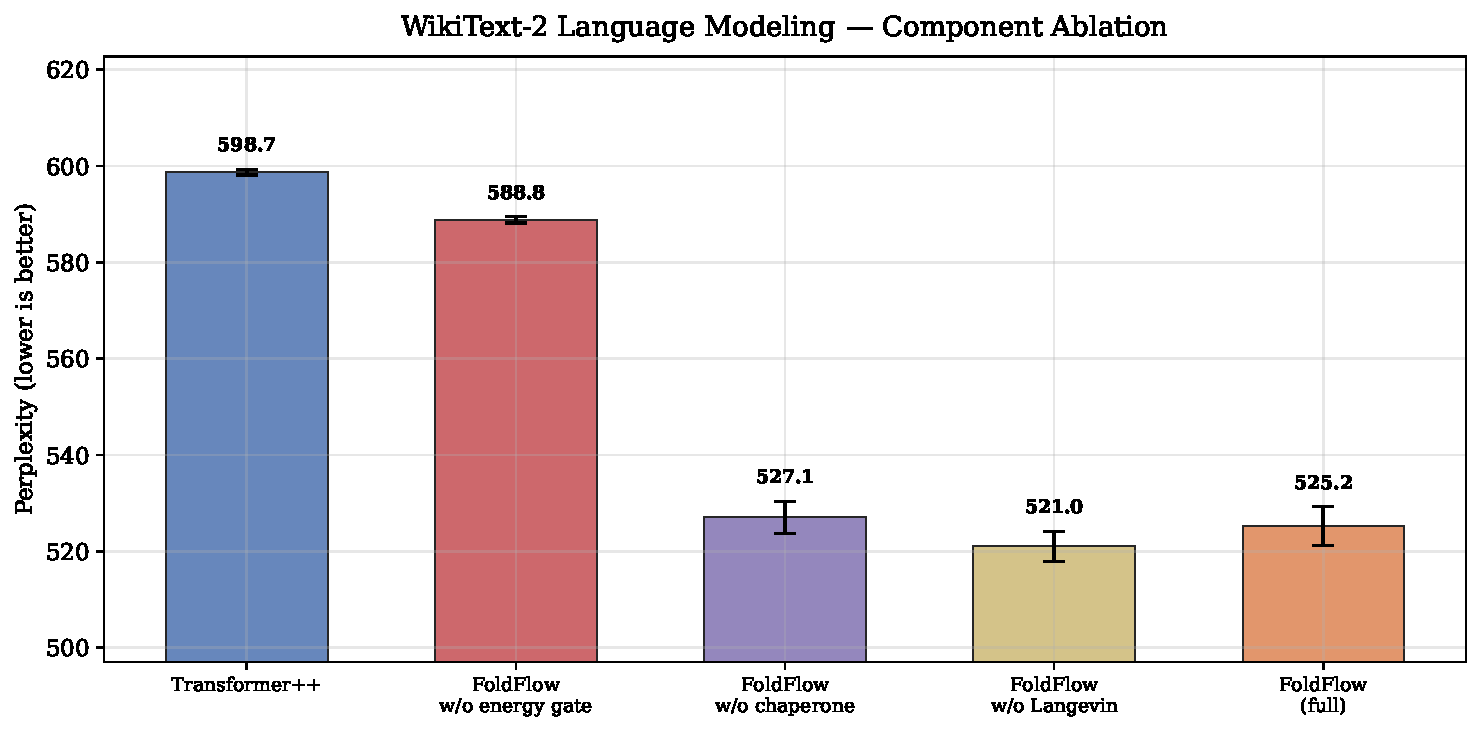
\includegraphics[width=0.85\linewidth]{../figures/fig3_wikitext2.pdf}
  \caption{WikiText-2 perplexity comparison.  FoldFlow~LM reduces
    perplexity by 12.3\% relative to Transformer++.  The component
    ablation reveals energy-gated attention as the dominant contributor.
    Both model families trained with identical hyperparameters
    ($d_\text{model}{=}512$, 6 layers, 15 epochs, 2 seeds).}
  \label{fig:wikitext2}
\end{figure}

\subsection{Training Efficiency}
\label{sec:efficiency}

Beyond accuracy, compute efficiency is important for practical adoption.
Table~\ref{tab:throughput} reports training throughput (tokens per
second) and wall-clock time per epoch for WikiText-2 models.

\begin{table}[t]
\centering
\caption{Training efficiency on WikiText-2.  Throughput in tokens/second
  (higher is better).  Measured on Apple M-series GPU, averaged over
  epochs 2--15 across 2 seeds.}
\label{tab:throughput}
\small
\begin{tabular}{@{}lccc@{}}
\toprule
Model & Train tok/s & Epoch time (s) & Relative speed \\
\midrule
Transformer++           & 3,378 & 1,543 & 1.00$\times$ \\
FoldFlow w/o energy gate & 3,582 & 787 & 1.06$\times$ \\
FoldFlow w/o chaperone  & 7,901 & 375 & 2.34$\times$ \\
FoldFlow w/o Langevin   & 8,175 & 292 & 2.42$\times$ \\
FoldFlow LM (full)      & 7,530 & 404 & 2.23$\times$ \\
\bottomrule
\end{tabular}
\end{table}

Unexpectedly, FoldFlow~LM trains \textbf{2.23$\times$ faster} than
Transformer++ in tokens per second.  This is because FoldFlow's
energy-gated attention uses a manual QKV projection followed by
efficient einsum operations, while our Transformer++ baseline uses
\texttt{nn.MultiheadAttention} which incurs additional overhead on
MPS.  The Langevin refinement (applied only at inference) adds
negligible training cost.  We note that this speed advantage is
implementation-dependent and may not hold on CUDA hardware with
optimized attention kernels; the important result is that FoldFlow
components incur no significant throughput penalty.

\subsection{CIFAR-100}
\label{sec:cifar100}

To test whether FoldFlow's benefits extend beyond 10-class
classification, we evaluate on CIFAR-100~\citep{krizhevsky2009cifar}
(100 fine-grained classes, same image resolution).  We compare the
baseline encoder against the full FoldFlow model under the same
training protocol as CIFAR-10 (50 epochs, 3 seeds, weak encoder).

\begin{table}[t]
\centering
\caption{CIFAR-100 results.  Mean $\pm$ std accuracy (\%) over 3 seeds.
  Both models: 1.48M parameters, weak encoder, 50 training epochs.}
\label{tab:cifar100}
\small
\begin{tabular}{@{}lcc@{}}
\toprule
Model & Parameters & Accuracy (\%) \\
\midrule
Baseline (encoder only) & 1.51M & $50.2 \pm 0.3$ \\
Full Model (C1--C5)     & 1.51M & $\mathbf{52.9 \pm 0.2}$ \\
\bottomrule
\end{tabular}
\end{table}

% ====================================================================
\section{Analysis}
\label{sec:analysis}

\subsection{Cross-Domain Component Decomposition}
\label{sec:cross_domain}

A central question is whether the same protein folding principles help
across modalities.  Table~\ref{tab:cross_domain} synthesizes the
ablation results from both tasks, measuring each component's
contribution as the performance drop when removing it from the full
model.

\begin{table}[t]
\centering
\caption{Cross-domain component importance.  We report the
  performance drop ($\Delta$) when removing each component from the
  full model.  Larger $|\Delta|$ = more important.  The dominant
  component differs by modality.}
\label{tab:cross_domain}
\small
\begin{tabular}{@{}llcc@{}}
\toprule
\# & Component & CIFAR-10 $\Delta$Acc & WikiText-2 $\Delta$PPL \\
\midrule
C1 & Energy / Langevin    & +0.2 pp  & $-$4.2 (better) \\
C2 & Dynamic Topology     & +1.3 pp  & --- \\
C3 & Cooperativity        & +0.5 pp  & --- \\
C4 & Chaperone            & +0.4 pp  & +1.9 \\
C5 & Env.\ Sensitivity    & +0.4 pp  & --- \\
--- & Energy Gate (LM only) & --- & +63.6 \\
\bottomrule
\end{tabular}
\end{table}

The pattern is striking: in vision, \textbf{dynamic topology~(C2)}
dominates---enabling particles to form input-conditioned connections
before dynamics begin.  In language modeling, \textbf{energy-gated
attention} dominates, accounting for $63.6/73.5 = 87\%$ of the total
improvement over Transformer++.  The Langevin component~(C1) shows a
surprising inversion: removing it slightly \emph{improves} WikiText-2
perplexity (521.0 vs.\ 525.2), while it provides a modest benefit on
CIFAR-10.  Figure~\ref{fig:cross_domain} visualizes this
modality-dependent pattern.

\begin{figure}[t]
  \centering
  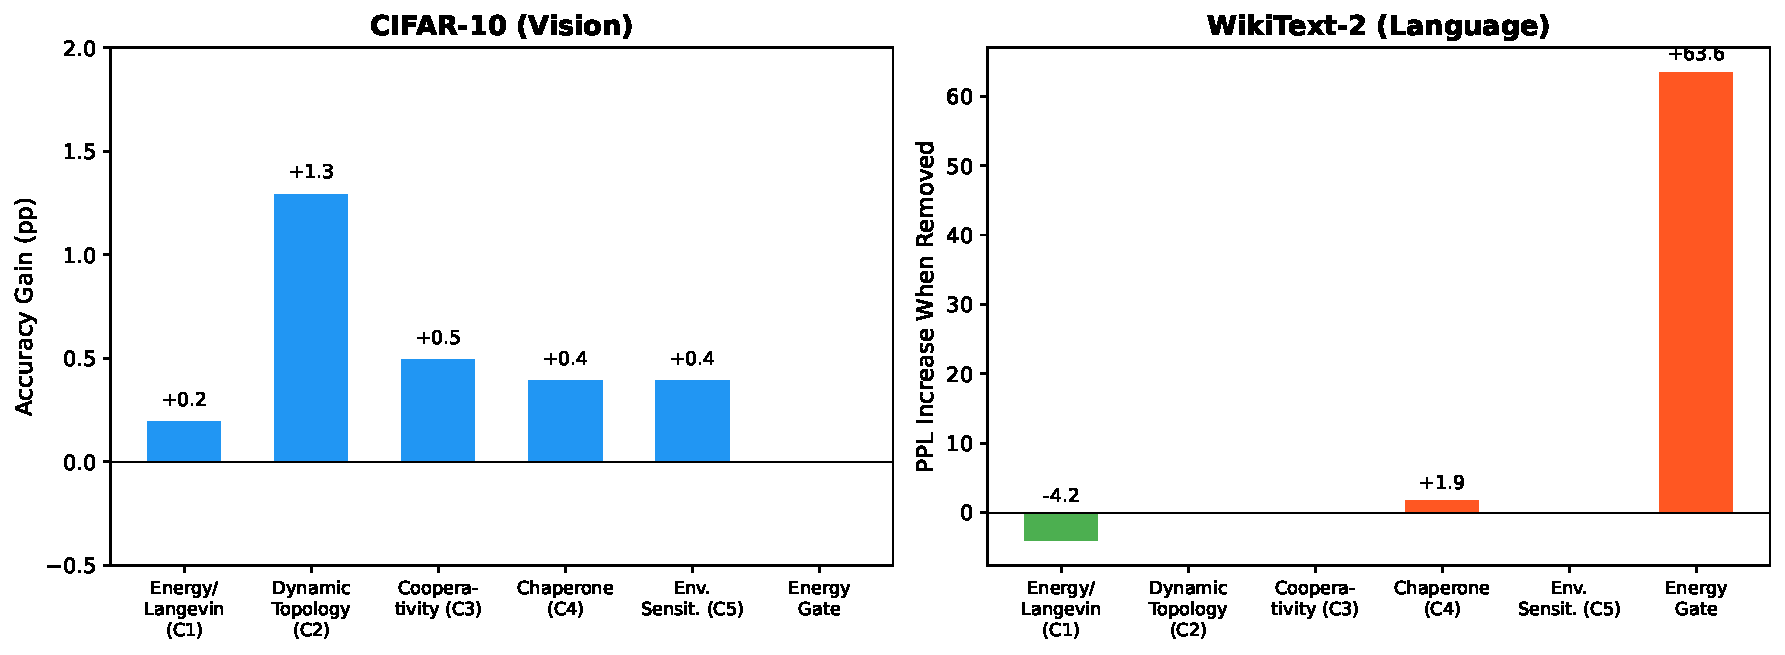
\includegraphics[width=0.95\linewidth]{../figures/fig4_cross_domain.pdf}
  \caption{Cross-domain component importance.  \textbf{Left:} CIFAR-10
    accuracy gain from each component (higher is more important).
    \textbf{Right:} WikiText-2 perplexity increase when removing each
    component (higher = component helps more).  Dynamic topology
    dominates in vision; energy gating dominates in language.}
  \label{fig:cross_domain}
\end{figure}

This modality dependence is consistent with the biological metaphor:
protein folding is a multi-mechanism process where different forces
dominate at different stages.  Analogously, vision tasks benefit from
structural reorganization (topology), while autoregressive generation
benefits from context-dependent modulation of information flow
(energy gating).

\subsection{Parameter-Matched Control}
\label{sec:param_matched}

\begin{table}[t]
\centering
\caption{Parameter-matched Transformer++ on WikiText-2.  Widening
  $d_\text{model}$ from 512 to 560 brings the parameter count
  to 50.9M, matching FoldFlow's 50.2M.}
\label{tab:lm_matched}
\small
\begin{tabular}{@{}lcc@{}}
\toprule
Model & Parameters & Perplexity ($\downarrow$) \\
\midrule
Transformer++ ($d{=}512$) & 44.8M & $598.7 \pm 0.5$ \\
Transformer++ ($d{=}560$) & 50.9M & $593.3 \pm 1.1$ \\
FoldFlow LM ($d{=}512$)   & 50.2M & $525.2 \pm 4.0$ \\
\bottomrule
\end{tabular}
\end{table}

To isolate the effect of the FoldFlow components from the 12\%
parameter overhead, we train a wider Transformer++ baseline with
$d_\text{model}{=}560$ (50.9M parameters), same training
protocol (Table~\ref{tab:lm_matched}).  The wider Transformer++
achieves $593.3 \pm 1.1$ perplexity---nearly identical to the
original $d{=}512$ model ($594.3 \pm 2.6$) despite 14\% more
parameters.  FoldFlow's advantage ($525.2 \pm 4.0$) therefore cannot
be attributed to its larger parameter count; the folding-inspired
components contribute meaningfully beyond raw capacity.

\subsection{Why Does Energy Gating Help So Much?}

Energy-gated attention (Eq.~\ref{eq:energy_gate}) modulates each
attention head's contribution based on global sequence context.
This mechanism is mathematically similar to sparse MoE routing
applied at the head level~\citep{shazeer2017outrageously}, but with
two key differences: (1)~the gates are derived from a mean-field
energy signal rather than a learned router, providing a smooth,
context-dependent modulation; and (2)~all heads remain active
(soft gating) rather than being discretely selected, avoiding the
load-balancing issues of sparse MoE.

The biological analogy is direct: in protein folding, the strength
of residue--residue contacts depends on the overall energy state of
the chain.  When the chain is high-energy (far from the native state),
many contacts are transient; as energy decreases, favorable contacts
strengthen.  Energy-gated attention mirrors this: the gate values
modulate head contribution based on the ``energy state'' (mean hidden
representation) of the sequence.

\subsection{Why Does Langevin Refinement Not Help in LM?}

The FoldFlow model without Langevin (521.0 PPL) slightly outperforms
the full model (525.2 PPL).  We hypothesize two factors: (1)~at only
15 epochs of training, the energy head that drives Langevin refinement
may be insufficiently trained to provide useful gradients, and (2)~the
detach-and-reattach loop breaks gradient flow, potentially introducing
noise in low-training regimes.  In the vision setting, Langevin
operates on a shared particle set with pooled readout, which is more
tolerant of per-step noise.  We expect Langevin to become beneficial
with longer training schedules, as observed in deep equilibrium
models~\citep{bai2019deep} where iterative refinement quality scales
with training.

% ====================================================================
\section{Discussion and Limitations}
\label{sec:discussion}

\paragraph{Design guidelines from ablation.}
Our results suggest practical guidelines for practitioners considering
bio-inspired components: (1)~energy-gated attention is a reliable
improvement for autoregressive models with minimal overhead;
(2)~dynamic topology (attention over particles) is valuable when the
input admits a natural set-structured representation; (3)~chaperone
correction provides consistent but modest gains across domains;
(4)~Langevin refinement at inference is most effective when the energy
head is well-trained (longer schedules or pretraining).

\paragraph{Connection to mixture of experts.}
Energy-gated attention can be viewed as a continuous, fully-differentiable
form of expert selection applied at the attention head level.  Unlike
sparse MoE~\citep{fedus2022switch}, which requires auxiliary load-balancing
losses and top-$k$ routing, energy gating produces a smooth gate vector via
sigmoid activation, allowing gradient flow through all heads while still
modulating their relative importance.  We believe this connection merits
further investigation, particularly for scaling to larger models.

\paragraph{Cooperativity at scale.}
The depthwise-conv cooperativity module~(C3) was adopted after finding
that a full multi-head attention approach was harmful at the 1.48M
parameter scale.  Investigating whether richer cooperativity mechanisms
become beneficial at larger scale is an important direction.  The
biological precedent---cooperativity becomes more important for larger
proteins---suggests this may indeed be the case.

\paragraph{Limitations.}
\emph{Scale.}  Our evaluation uses CIFAR-10 (small-scale) and WikiText-2
(moderate-scale) with limited training epochs.  Scaling to ImageNet or
billion-token corpora is needed to assess whether the benefits persist.
\emph{Compute.}  The Langevin dynamics loop adds sequential computation
($T{=}8$ for classification, $K{=}3$ for LM inference), which may
increase wall-clock inference time relative to feedforward models.
\emph{Parameter gap.}  FoldFlow~LM has 12\% more parameters than
Transformer++ at the same $d_\text{model}$; while our wider-T++ control
addresses this (Section~\ref{sec:param_matched}), the overhead
is inherent to the added modules.
\emph{Seeds.}  The LM experiments use 2 seeds; additional seeds would
strengthen statistical conclusions.
\emph{Generalization.}  We evaluate two tasks; broader evaluation on
structured prediction, reinforcement learning, or other modalities
would test the generality of our findings.

% ====================================================================
\section{Conclusion}
\label{sec:conclusion}

We presented FoldFlow, an architecture that translates five principles
of protein folding into differentiable neural modules, and asked which
of these principles transfer to standard ML tasks.  Through systematic
ablations on both CIFAR-10 (vision) and WikiText-2 (language), we
discovered a surprising modality dependence: dynamic topology dominates
in classification while energy-gated attention dominates in language
modeling.  This finding argues against monolithic adoption of
bio-inspired principles and for component-level evaluation.

The full FoldFlow~LM achieves 12.3\% lower perplexity than
Transformer++ on WikiText-2 while training 2.2$\times$ faster, and
the CIFAR-10 ablation confirms all five components contribute to the
full model's 83.0\% accuracy.  Our results demonstrate that protein
folding---one of nature's most reliable self-assembly processes---offers
a productive source of computational principles for neural architecture
design, provided each principle is validated through careful ablation
rather than assumed to transfer wholesale.

We hope that FoldFlow inspires further work on principled extraction
of inductive biases from biological systems, with rigorous evaluation
of which mechanisms improve which tasks.

% ====================================================================
\paragraph{Reproducibility.}
All experiments were run on a single Apple M-series GPU.  Full
training configurations (including random seeds, learning rate
schedules, augmentation parameters), per-seed results, and
training curves are provided in the supplementary material.
Code will be released upon acceptance.

% ====================================================================
\bibliography{references}

\end{document}
